\chapter{Method}
\section{Radial velocity components in linear theory}\label{sec:radlintheory}
One of the goals of this project is to test the viability of using the assumptions
from linear theory and study wether it is a good physical approximation for
studying the physics of voids and filaments. The radial velocity component of
halos in filaments and voids is an analytical tool that is useful for comparing
with data from simulation for testing wether linear theory can be used to
approximate the physical behaviour of halos and galaxies observed in these objects.
\subsection{Radial velocity component for filaments}\label{sec:filamentvr}
When calculating the radial velocity component of filaments, the average filament is
approximated to be a cylindrical object. The radial component is the component of
the velocity vector $\vec{v}$ that points perpendicular to the longitudinal axis
$L$. This is illustrated in figure \ref{fig:filamentvr}. For this analysis we
will assume that the other velocity components are negligible and that the
radial component is the significant component.
\begin{figure}\label{fig:filamentvr}
    \begin{tikzpicture}
        \draw[->] (-4,0,0) -- (4,0,0) node[below right] {$L$};
        \draw[->] (0,1,0) -- (0,0.5,0) node[below right] {$v_r$};
        \draw[->] (0,-1,0) -- (0,-0.5,0) node[below right] {$v_r$};
        \node (A) [draw, cylinder, shape aspect=1.8, minimum height=50mm, minimum width=20mm] {};
    \end{tikzpicture}
    \caption{Illustration of a cylindrical filament with longitudinal axis $L$ and radial velocity component $v_r$.}
\end{figure}
in linear theory can be written as
\begin{equation}\label{eq:lincont}
    \frac{d\delta}{dt}+\frac{1}{a}\nabla\cdot\vec{v}=0.
\end{equation}
 The continuity equation In linear theory one can write
 $d\delta/dt=Hf\delta$ \cite[p.~347]{schneider2006extragalactic}, where $f$ is the growth factor
defined in equation \ref{eq:growthfac}. Substituing this into equation
\ref{eq:lincont} one will get
\begin{equation}\label{eq:templineq}
    \nabla\cdot\vec{v}=-Hfa\delta.
\end{equation}
Assuming cylindrical coordinates we can replace the
divergence
\begin{equation}
    \nabla\cdot\vec{v}=\frac{1}{r}\frac{\partial}{\partial r}(rv_r)+\frac{1}{r}\frac{\partial v_\phi}{\partial \phi} +\frac{\partial v_L}{\partial L}.
\end{equation}
Assuming that the radial component $v_r$ gives the significant contribution and
the two other are negligible, by inserting into equation \ref{eq:templineq} on
will get
\begin{equation}
    \frac{1}{r}\frac{\partial}{\partial r}(rv_r)=-Hfa\delta.
\end{equation}
Multiplying both sides by $r$ and integrating one will be left with
\begin{equation}
    v_r=-\frac{1}{r}Hfa\int_0^r\delta(x) x dx.
\end{equation}
By defining the average mass density contrast for filaments $\Delta_f(r)$
as
\begin{equation}\label{eq:contrastfil}
    \Delta_f(r)=\frac{2}{r^2}\int_0^r\delta(x) x dx,
\end{equation}
one can write the radial velocity component for a halo in a filament as
\begin{equation}\label{eq:vrfilament}
    v_r(r) = -\frac{1}{2}Hfar\Delta_f(r).
\end{equation}
\subsection{Radial velocity component for voids}
The radial velocity component for voids is similar to the one for filaments
except that for voids one assumes a spherical coordinate system. This assumption
is based on the notion that the average void should have a spherical shape with,
on average, no prefferred direction for overdensities on the rim and
thereby having a spherical density profile. Since objects cluster towards larger
densities, approximating the velocity of halos and galaxies around
voids to be dominated by the radial component, moving straight away from the
underdensity in the center of the void one can argue that the radial velocity
should be the dominating component. This is illustrated in figure \ref{fig:filamentvr}.
\begin{figure}\label{fig:filamentvr}
    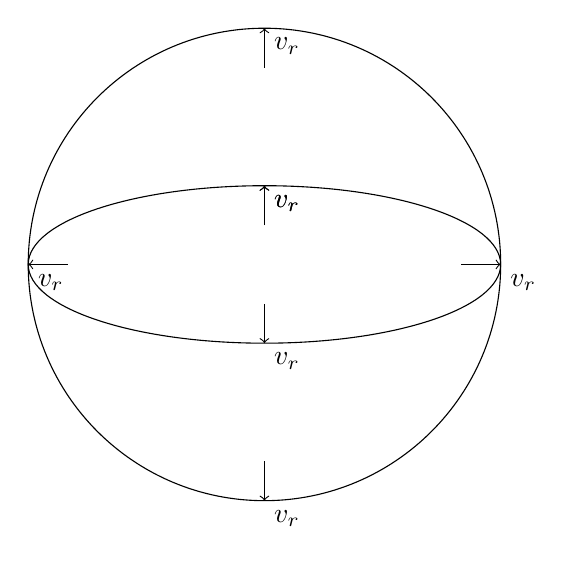
\begin{tikzpicture}
        \draw[->] (0,0.5,0) -- (0,1,0) node[below right] {$v_r$};
        \draw[->] (0,-0.5,0) -- (0,-1,0) node[below right] {$v_r$};
        \draw[->] (0,0.5,0) -- (0,1,0) node[below right] {$v_r$};
        \draw[->] (2.5,0,0) -- (3,0,0) node[below right] {$v_r$};
        \draw[->] (-2.5,0,0) -- (-3,0,0) node[below right] {$v_r$};
        \draw[->] (0,2.5,0) -- (0,3,0) node[below right] {$v_r$};
        \draw[->] (0,-2.5,0) -- (0,-3,0) node[below right] {$v_r$};
        \draw (0,0) circle (3cm);
        \draw (0,0) ellipse (3cm and 1cm);
    \end{tikzpicture}
    \caption{Illustration of a spherical void with radial velocity pointing outwards from the center of the void.}
\end{figure}
The derivation for the radial velocity component is the same for voids as for
filaments up until equation \ref{eq:templineq}. The difference for voids is that
the divergence now has to be calculated in spherical coordinates given by
\begin{equation}
    \nabla\cdot \vec{v}=\frac{1}{r^2}\frac{\partial}{\partial r}(r^2v_r)
                       +\frac{1}{r\mathrm{sin}\theta}\frac{\partial}{\partial r}(\mathrm{sin}\theta v_\theta)
                       +\frac{1}{r\mathrm{sin}\theta}\frac{\partial}{\partial r}(\phi v_\phi).
\end{equation}
As for filaments only the radial component is assumed to be non-negligible
giving
\begin{equation}
    \frac{1}{r^2}\frac{\partial(r^2v_r)}{\partial r}=-Hfa\delta.
\end{equation}
Multiplying by $r^2$ and integrating one will get
\begin{equation}
    v_r = -\frac{1}{r^2}Hfa\int_0^r x^2\delta(x)dx.
\end{equation}
As for filaments a average mass density contrast for voids is defined as
\begin{equation}\label{eq:contrastvoid}
    \Delta_v(r)=\frac{3}{r^3}\int_0^r x^2\delta(x)dx,
\end{equation}
which will give an expression for the radial velocity for voids
\begin{equation}\label{eq:vrvoid}
    v_r(r)=-\frac{1}{3}Hfar\Delta_v(r).
\end{equation}
\subsection{Minor correction term to velocity around voids.}\label{sec:vr_correction}
The equation for the radial velocity around voids given by \ref{eq:vrvoid} is a simple modelling of the velocity using a pure geometrical interpretation. I will implement and test wether adding a correction term to equation \ref{eq:vrvoid} of halos around voids proposed by \cite{Achitouv_streaming} will provide better fits to data. The proposed model adds a correctional term to the velocity given as
\begin{equation}\label{eq:achitouv2017}
    v(r)=-\frac{1}{3}Hfar\Delta_v(r)+\Gamma\frac{6}{7}faH\frac{r}{6}\Delta_v^{(2)},
\end{equation}
where $\Gamma=+1$, when $\Delta_v(r)>0$ and $\Gamma=-1$, when $\Delta_v(r)<0$. In addition to the mass density contrast for voids $\Delta_v(r)$ defined in equation \ref{eq:contrastvoid} an additional $\Delta_v^{(2)}$ is introduced as 
\begin{equation}
    \Delta_v^{(2)}(r)\equiv\frac{3}{r^3}\int_0^rx^2\delta(x)^2dx.
\end{equation}
This semi-empirical term is motivated by including a modified second order eularian perturbation term in velocity (eq. (43) in \cite{Catelan_2ndordervelpert})
\begin{equation}
    \nabla\cdot v^{(2)}=\frac{3}{7}f_2aH(\delta^{(1)})^2+\text{Other terms}.
\end{equation}
This modification to the velocity model will be tested by fitting parameters with data when calculating the cross correlation function derived later in section \ref{sec:vgcrosscorr}.
\section{Numerical measurement of correlation functions and multipole expansions.}\label{sec:numerical_corr}
As mentioned in section \ref{sec:corrtheory} correlation functions are useful
tools for measuring the statistical properties of the universe. In order to test
analytical models one has to compare with data from observations or simulations.
The code \footnote{The code for measuring correlation functions utilized for this analysis can be found at \url{https://github.com/seshnadathur/pyCUTE}.} used for this project to measure angular correlation functions
implements a Landy-Szalay estimator \cite{Landy}. The Landy-Szalay estimator
for the angular cross correlation function, where $s$ denotes redshiftspace, reads
\begin{equation}
    \xi^s(s,\mu)=\frac{\langle D_1D_2\rangle-\langle D_1R_2\rangle-\langle D_2R_1\rangle+\langle R_1R_2\rangle}{\langle R_1R_2\rangle}.
\end{equation}
Where, the terms in the square brackets denotes the number of pairs of the given quantities. In this analysis, subscript $1$ denotes either void centers or center or
the center of cosmic filaments and subscript $2$ denotes halo positions. $D_1$
and $D_2$ refers to the actual data while $R$ is samples from a random
distribution resembling the dataset. Each quantity in the squared brackets
denote the mean value of of a pair with separation $r$ and $\mu$, where
$\mu=cos(\theta)$ is the cosine of the angle between the separation vector and
the line of sight direction. However in this project I will only deal with simulation data in which includes a complete catalogue without empty patches.
The numerical calculation of the correlation function will then consist of counting void-halo pairs with separation $s$ and angle $\mu$.
An illustration of a pair in the coordinate system
of the observer is illustrated in figure \ref{fig:corrpair}
\begin{figure}\label{fig:corrpair}
    \begin{tikzpicture}
        \def\myrad{2}% radius of the circle
        \def\myang{60}% angle for the arc
        %\draw (0,0) -> (10,0) {s};
        % the origin
        \coordinate (O) at (10,0);
        
        \draw[line width=0.2mm][->] (0,0) -- (10,0);
        \draw[line width=0.2mm][->] (10,0) -- (10-1.414,-1.414);
        \draw[line width=0.2mm][->] (0,0) -- (10-1.414,-1.414);
        % the circle and the dot at the origin
        \node[text width=10cm] at (13.3,0.5) {Filament/void center};
        \node[text width=10] at (5,0.5) {$\vec{r}_{void/filament}$};
        \node[text width=10] at (9.5,-1.4) {$\vec{r}$};
        \node[text width=10] at (5,-1.1) {$\vec{r}_{halo}$};
        \node[text width=5] at (0,1) {Observer};
        \node[text width=5] at (3.7,-1.1*0.34) {$\theta$};
        \draw (O) node[circle] {} circle [radius=\myrad];
        % the ``\theta'' arc
        \draw (O) [thick,domain=330:360] plot ({2+cos(\x)}, {sin(\x)});
    \end{tikzpicture}
    \caption{Figure illustrating the system used in this analysis. This
    figure is drawn in realspace thereby all vectors denoted as $\vec{r}$.
    Transformation to redshiftspace will distort the galaxy positions and the
    corresponding system has vectors denoted as $\vec{s}$.}
\end{figure}
\\\indent
In realspace, due to isotropy and homegenity, there is no angular dependence on the correlation function and $\xi^r(r)$ is only a function of radius. However the redshiftspace distortions themselves are responsible for the angular dependency in $\xi^s(r,\mu)$. Since redshiftspace distortions are only present when considering the component of a vector parallel to the line of sight direction, we loose isotropy in redshiftspace. In order to characterise the angular dependencies the angular cross correlation function is expanded into multipoles
\begin{equation}
    \xi^s_\ell(s)=\int_0^1\xi^s(s,\mu)(1+2\ell)L_\ell(\mu)d\mu
\end{equation}
\cite{Nadathur_corr}, where $L_\ell(\mu)$ are Legendre polynomials
of order $\ell$. The redshiftspace distortions themselves are fully characterised by the monopole and quadrupole terms\cite{Hamaus_2017}. The Legendre polynomials for $\ell=0$ and
$\ell=1$ are given by
\begin{equation}
    L_0(\mu)=1
\end{equation}
and
\begin{equation}
    L_2(\mu)=(3\mu^2-1)/2.
\end{equation}
\section{Void Analysis}
\subsection{Density profile}\label{sec:voiddensity}
After running the void finding algorithm from REVOLVER on our dataset we have a list of $x$, $y$
and $z$ coordinates for every void center. With a catalogue of void centers one
has to compare their position to the galaxy catalogue in which they are found to
calculate the average density profile as a function of distance from the void
center. Using a periodic kd-tree module \footnote{The periodic kd-tree code
applied for this analysis is found at at \url{https://github.com/patvarilly/periodic_kdtree}} to search for
the nearest halos of the void centers with a gradually increasing radius one can count the halos in
the catalogue close to a given void center. For every void a search for
neghbouring halo particles is conducted with a gradually increasing radius. For
a linearly spaced radius array $\vec{r}=\{r_0,\dots,r_{n}\}$ using an iterative
approach every galaxy in a sphere with radius $r_{i}$, where
$i\in\mathbb{N}\bigcap [r_0,r_{n}]$ denotes the
number of iterations, is counted. The total number of halos is stored for
every iteration. For the first iteration the number of halos in a sphere around the void
center is calculated and stored. The density for this sphere is then $n_i/V_i$,
where $n_i$ is the number of halos inside the sphere and $V_i=4\pi r_{i}^3/3$. For
the next iteration the number of halos inside a sphere with radius $r_{i+1}$ is
counted. Alot of the halos inside this new sphere overlaps with the previous
sphere. Therefore the number of halos in the previous step were stored and then
subtracted from the number of galaxies in the new sphere leaving only the number
of halos counted in the spherical shell that does not overlap between the two
spheres. The volume of this spherical shell is $V_{i+1}=4\pi(r_{i+1}^3-r_i^3)/3$. The
number density in the shell defined by subtracting the previous sphere from the
new sphere is the number of galaxies in the new sphere subtracted by the number
of galaxies in the previous sphere divided by the volume of the sperical shell.
The total number of galaxies in the new sphere is stored and this process is
repeat for all iterations defined by the radius vector $\vec{r}$. This process
will give the density profile as a function of radius for a given void. By
adding the density profiles for all voids and diving by the number of voids one
will get an average density profile for the whole dataset. From the relation for the overdensity, given by equation \ref{eq:overdensity},
stacked overdensity for the voids in a catalogue is given by thte relation
\begin{equation}
    \delta(r)=\rho(r)/\bar{\rho}-1,
\end{equation}
where $\bar{\rho}$ is the average density in the simulation volume $N/V$, where $N$ is the total number of halo particles in the halo catalogue
and $V$ is the total volume, which in this case is $2500^3$ [$\mathrm{Mpc}^3/h^3$]. The number of particles for the datasets tested is given in table \ref{tab:MDproperties}. 
\subsection{Velocity profile and velocity dispersion}\label{sec:voidvel}
When studying linear theory applied to voids and filaments, one needs an observational or
numerical representation to test its validity. As explained in section
\ref{sec:radlintheory} the radial velocity profile can be represented analytically and
may provide a good comparison. In addition to the $x$, $y$ and $z$ coordinates for the
halo particles, the galaxy catalogue used also containts the $v_x$, $v_y$ and
$v_z$ particles. The radial velocity profile is calculated in a
similar manner as the density profile for voids described in
\ref{sec:voiddensity}. Using a periodic kd-tree centered at the current void one
can count all particles in a sphere around the current void center. For a given
halo particle its position with respect to a given void center is given by
\begin{equation}\label{eq:voidpos}
    \vec{r}=\vec{r}_{\mathrm{void}}-\vec{r}_{\mathrm{halo}}.
\end{equation}
This is the vector that points radially from the void center to a given halo
particle. The radial velocity component is is the component of the velocity of a
given halo particle $\vec{v}$ that points along this vector. The component of vector
$\vec{v}$ along vector $\vec{r}$ is caluclated as
\begin{equation}
    v_r=\frac{\vec{r}\cdot\vec{v}}{\vert\vec{r}\vert}.
\end{equation}
This is the radial velocity for a halo particle with respect to a given void
center. In a similar manner to the density profile the radial velocity is
calculated iteratively for every particle in sphere around the void center. In
order to get the radial velocity profile the particles are divided into
shells. For every iteration, for a given void, for each sphere the radial
velocity is stored for the next iteration. The radial velocity in a given shell
for the next iteration is the radial velocity in the new sphere subtracted by
the radial velocity in the previous sphere. This is averaged by, for each shell,
dividing by the number of particles in a given shell. After this has
been done for all voids the radial velocity profile is divided by the number of voids in the catalogue to get
the average radial velocity profile for a single halo particle in the catalogue.
\\\indent
The velocity dispersion $\sigma_v$ is also calculated. The velocity dispersion
is given by the usual expression for the standard devation
\begin{equation}\label{eq:sigma_v}
    \sigma_{v} = \sqrt{\langle v^2 \rangle - \langle v\rangle^2}.
\end{equation}
This velocity is along the line of sight for the observer. Since i am working with data from simulations
The observer is located in the $xy-$plane and all velocites are measured in the $z-$direction. In real observations
the observer would be located at a point and an angular dependency would be introduced.
Therefore in this analysis only the $v_z$ component
is considered. This is calculated in spherical shells around each void center to
get the average void velocity dispersion profile.
\subsection{Void-galaxy cross correlation function.}\label{sec:vgcrosscorr}
As mentioned in section \sec{sec:corrtheory} correlation functions are
essential tools in cosmology for measuring the statistical properties of
observables in the universe. In this analysis one of the cross correlations that
will be looked into is the cross correlation between void centers and galaxies
or halos. Following the approach of \cite{Nadathur_corr}, the following
subsection will describe how to derive the void-galaxy cross correlation
function. 
\\\indent
Let $\vec{r}_{void}$ denote the position of a void center and $\vec{r}_{halo}$ denote the
position of a halo or galaxy particle in realspace. Their separation vector $\vec{r}$ is then
given by equation \ref{eq:voidpos}. A figure of the system is illustrated in \ref{fig:corrpair}. The relation from redshiftspace to realspace
is given as
\begin{equation}\label{eq:s_to_r}
    \vec{s}=\vec{r}+\frac{\vec{v}_{pec}\cdot\hat{r}_{void}}{aH}\hat{r}_{void},
\end{equation}
where $v_{pec}$ is the peculiar velocity of a galaxy or halo particle and
$\hat{r}_{void}=\vec{r}_{void}/ \vert \vec{r}_{void}\vert$. Here it is assumed
that the velocity of void centers are negligible. In redshiftspace the distribution of galaxies or halos gets distorted and therefore,the number of voids in
realspace may not be preserved in redshiftspace. Since, for this project, data from simulations are utilized one has access to both a catalogue with realspace and redshiftspace positions. If one utilizes observational data only the redshiftspace positions are observed. Therefore reconstruction,
described here in section \ref{sec:reconstruction}, has to be applied to regain
the field in realspace from redshiftspace if observational data is used. By using the realspace and redshiftspace catalogues provided by the Multidark simulations\cite{Multidark_dataset}, as i will do in this project, one eliminates errors introduced by the additional step of performing reconstruction on the redshiftspace data. However, for future work, it is important to study the effect of performing this extra step on simulation data to better quantify the potential error introduced as this step has to be done for this method to be applied on observational data.\\\indent
The basic assumption when calculating the cross correlation function
required is that the number of void-galaxy pairs in the simulation volume is
unchanged during transformation from realspace to redshiftspace. This is stated
mathematically as
\begin{equation}\label{eq:corr_void_start}
    (1 + \xi^s_{\mathrm{vg}}(\vec{s}))\mathrm{d}^3\mathrm{s}=(1 + \xi^r_{\mathrm{vg}}(\vec{r}))\mathrm{d}^3\mathrm{r},
\end{equation}
where superscript $r$ and $s$ denotes realspace and redshiftspace respectively.
Here $\xi^s_{vg}(\vec{s})$ is the cross correlation between realspace voids and
the redshifted galaxy field and $\xi^r_{vg}(\vec{r})$ is the cross correlation
between realspace voids and realspace galaxy positions. $\vec{r}$ and $\vec{s}$
are vectors pointing from the void center to a given galaxy position in
realspace and redshiftspace respectively. Another assumption made
is that the velocity of all halo particles near a void can be approximated by
its radial velocity $\vec{v}=v_r \hat{r}$. We orient our coordinate system so that
$\hat{r}_{void}=\hat{z}$. The observer will then only experience redshift
distortions in the $z$ direction. This makes $s_x=r_x$ and $s_y=r_y$. With $\hat{r}_{void}=\hat{z}$ then have that
$\hat{r}_{void}\cdot\hat{r}=z/r$. We can then rewrite equation \ref{eq:s_to_r}
as
\begin{equation}\label{eq:s_tp_r}
    \vec{s}=\vec{r}+\frac{v_rz}{aHr}\hat{z}.
\end{equation}
The coordinate transformation will then have the
following jacobian determinant
\begin{equation}
    \vert J(\frac{s}{r})\vert=
    \begin{vmatrix}
        1 & 0 & 0\\
        0 & 1 & 0\\
        0 & 0 & \frac{\partial s_z}{\partial r_z} 
    \end{vmatrix},
\end{equation}
where
\begin{equation}
    \frac{\partial s_z}{\partial r_z} = 1 + \frac{v_r}{raH}+\frac{(v_r^\prime-v_r/r)}{aH}\mu^2.
\end{equation}
here $v_r^\prime$ denotes derivative with respect to $r$. One can now rewrite
equation \ref{eq:corr_void_start} as
\begin{equation}\label{eq:corr_temp}
    1 + \xi^s_{\mathrm{vg}}(\vec{s})=(1 + \xi^r_{\mathrm{vg}}(\vec{r})) \Big[1 + \frac{v_r}{raH}+\frac{(v_r^\prime-v_r/r)}{aH}\mu^2 \Big]^{-1}.
\end{equation}
This equation can be calculated using both the velocity derived from linear theory from voids, given by equation \ref{eq:vrvoid}, and the modified velocity proposed by \cite{Achitouv_streaming} given in equation \ref{eq:achitouv2017}.
\\\indent
Using the radial velocity $v_r$ for halos derived from linear theory, given in equation \ref{eq:vrvoid}, it is customary to approximate the expression for the cross correlation function given in equation \ref{eq:corr_temp}. In addition to the radial velocity $v_r$ We have $\Delta_v^\prime(r)=3(\delta(r)-\Delta_v(r))/r$ giving
\begin{equation}
    v_r^\prime=-Hfa(\delta(r)-\Delta(r)),
\end{equation}
where $\Delta_v(r)$ is the density contrast defined in equation
\ref{eq:contrastvoid}. Inserting this into equation \ref{eq:corr_temp} results
in
\begin{equation}\label{eq:corr_temp2}
    1 + \xi^s_{\mathrm{vg}}(\vec{s})=(1 + \xi^r_{\mathrm{vg}}(\vec{r})) \Big[1 -\frac{f}{3}\Delta(r)-f\mu^2(\delta(r)-\Delta(r))\Big]^{-1}.
\end{equation}
This equation can be expanded using the taylor expansion
$1/(1-x)\approx1+x+\mathcal{O}(x)^2$. When expanding this equation it is
appropriate with a review of the terms. It is
assumed that for voids the density profile is small enough so that terms of
second order in $\delta$ and $\Delta_{v}$ is negligible meaning $\delta^2$,
$\Delta_{v}^2$ and $\delta\Delta_v$ terms are not considered. This leaves us with terms
of order $\delta$ and  $\delta\xi^r$. Equation
\ref{eq:corr_temp2} then reduces to
\begin{equation}\label{eq:corr_no_stream}
    \xi^{s,base}_{\mathrm{vg}}(\vec{s},\mu)=\xi^r(r)+\frac{f}{3}\Delta_v(r)(1+\xi^r(r))+f\mu^2[\delta(r)-\Delta_v(r)](1+\xi^r(r)).
\end{equation}
This is an approximation to equation \ref{eq:corr_temp}. Allthough the approximations give
the model sufficient validity on a range of scales \cite{BeyondBAO}, testing during development of the methodology showed that the full expression given by equation \ref{eq:corr_temp} proved to correspond better with numerical calculations described in section \ref{sec:corrtheory}. Since the equations are implemented numerically there should therefore be no reason to not use the full expression for the sake of this analysis. Allthough 
as mentioned earlier, it is worth noting that since $\xi^r(r)$ is the correlation function in
realspace coordinates, if one is to apply this method to observational data
reconstruction, described in section \ref{sec:reconstruction}, has to be performed. Since observational data is observed in
redshiftspace, one cannot observe $\xi^r(r)$ directly. One therefore has to
perform reconstruction on the data and then perform the correlation function
calculation described in section \ref{sec:numerical_corr} in order to obtain
$\xi^r(r)$. When working with simulation data one has knowledge about the
particle field in redshiftspace and in realspace. In this analysis $\xi^r(r)$ is calculated by cross correlating the realspace catalogue with realspace voids using pyCUTE. 
\\\indent
The correlation function in redshiftspace $\xi^s_{\mathrm{vg}}(\vec{s},\mu)$
relies on the realspace length of the separation vector $\vert\vec{r}\vert$ as
can be seen from equation \ref{eq:corr_no_stream}. The system is illustrated in
figure \ref{fig:corrpair}. For every distance from the void center $s$ in
redshiftspace, we want the corresponding length from the void center $r$ in
realspace to calculate $xi^r_{\mathrm{vg}}(r)$, $\delta(r)$ and $\Delta_v(r)$.
To achieve this we start by decomposing $s$ into a parallel and perpendicual
component using basic trigonometry
\begin{equation}
    s_\parallel=s\mu
\end{equation}
and
\begin{equation}
    s_\perp=s(1-\mu^2).
\end{equation}
In the simulation volume there is only redshiftspace distortions along the line
of sight direction. This will mean that the perpendicual component is unchanged
when changing coordinates from redshiftspace to realspace. The parallel
component is found by inserting equation \ref{eq:vrvoid} into equation \ref{eq:s_to_r} and using the fact that there are no distortions in the perpendicular direction as
\begin{equation}
    r_\parallel=s_\parallel + s\frac{\beta\Delta(s)\mu}{3},
\end{equation}
where $\beta=f/b$.
The correspending realspace separation is then given as
\begin{equation}
    r=\sqrt{r_\parallel^2+r_\perp^2}.
\end{equation}
\subsection{Expanding model to account for velocity dispersion}
The previous model for the void-galaxy correlation function is a good
approximation. However it can be improved by taking into account the velocity
dispersion of galaxies around the void centers in the line of sight direction.
This will provide a more accurate model thereby giving a better fit to data.
Instead of only considering radial velocities another component along the line
of sight direction is added
\begin{equation}
    \vec{v}=v_r\hat{r}+v_\parallel \hat{r}_{void}.
\end{equation}
$v_r$ is the radial velocity used in the previous model given by equation
\ref{eq:vrvoid}. $v_\parallel$ is given by a gaussian probability distribution
$P(v_{\vert\vert})$ with zero mean
\begin{equation}\label{eq:gaussian_prop_corr}
    P(v_\parallel)=\frac{1}{\sqrt{2\pi}\sigma_{v_{\parallel}}}\mathrm{exp}\Big[-\frac{v_\parallel^2}{2\sigma_{v_\parallel}^2}\Big].
\end{equation}
Since in our simulation volume we only measure velocities along the line of
sight direction we can take $\sigma_{v_{\parallel}}$ to measured by equation
\ref{eq:sigma_v}. If this method is to be used on observation, one cannot necessariliy extract the velocities of the each particle and gain information about $\sigma_v$. Therefore simulations has to be utilized in order to calculate this quantity. This will however introduce free parameters when doing paremeters estimations as this profile has to be scaled differently when derived from another dataset. Using equation \ref{eq:gaussian_prop_corr} one will get an integral for calculating the improved
model taking into account dispersion in the velocity of halos \cite{BeyondBAO}
\begin{equation}\label{eq:corr_stream}
    1+\xi^{s,streaming}(s,\mu)=\int_{-\infty}^\infty\frac{1+\xi^{s,base}(s)}{\sqrt{2\pi}\sigma_{v_{\parallel}(r)}}\mathrm{exp}\Big[-\frac{v_\parallel^2}{2\sigma_{v_\parallel}^2(r)}\Big]dv_\parallel.
\end{equation}
\section{Filament Analysis}
\subsection{Masking the simulation volume}\label{sec:maskingfilament}
When applying the DisPerSE code on the particle distribution the output will be,
for each filament detected, coordinates to the start point of each segment
making up the total filament. For each filament there will be a number of
filament segments with startpoints $\vec{r}_i$. This also makes $\vec{r}_{i+1}$
the endpoint of filament with startpoins $\vec{r}_i$. Each filament segment $F_j$ is
then given by
\begin{equation}
    \vec{F}_{j}=\vec{r}_{i+1}-\vec{r}_i.
\end{equation}
Here $j$ denotes a given filament segment while $i$ denotes the startpoints of the
segments. With this notation $j+1$ is denoted by startpoints $i+2$ and $i+1$ and
so on. When a given filament segment is defined the simulation volume is masked
to remove all particles outside the edges of the start and endpoint of the
filament segment. This is done by defining  two planes perpendicular to
$\vec{F}_j$ with points $\vec{r}_{i+1}$ and $\vec{r}_i$. The equation for a
plane $P$ given a vector $\vec{F}$ and a point $\vec{r}$ is given
by the usual formula
\begin{equation}\label{eq:plane_mask}
    P=F_x(x-r_x)+F_y(y-r_y)+F_z(z-r_z)=0,
\end{equation}
where $x$, $y$ and $z$ are coordinates of the particles in the simulation
volume. In this section this vector will be denoted as $\vec{x}$.
The coordinates $r_x$, $r_y$ and $r_z$ are the components of $\vec{r}$.
For a given filament $F$ segment with startpoint $r_{i}$ and endpoint $r_{i+1}$ the particles kept are the particles
satisfying the following criteria
\begin{equation}
    P_0=F_x(x-r_{i_x})+F_y(y-r_{i_y})+F_z(z-r_{i_z})>0
\end{equation}
and
\begin{equation}
    P_1=F_x(x-r_{{i+1}_x})+F_y(y-r_{{i+1}_y})+F_z(z-r_{{i+1}_z})<0.
\end{equation}
The rest of the particles are masked keeping only the particles in the
simulation volume bound by the two plane parallel to the filament segment
centered in the startpoint and endpoint. A figure of this process is illustrated in figure \ref{fig:galaxy_catbbox}
\begin{figure}[htbp]
    \subfigure[]{\includegraphics[width=0.5\textwidth]{figures/catalogue_nocut.png}}\hspace{1em}%
    \subfigure[]{\includegraphics[width=0.5\textwidth]{figures/filament_cat_cut.png}}
    \caption{Figure illustrating visually how the the halo catalogue is masked. One the left is a scatter plot of the halo catalogue without a mask. The right figure illustrates the masking of the catalogue where the two red dots are the start and endpoints of the filament segment. Here one can see that only particles bound by the spine of the filament segment itself are kept. The dataset used for this illustration is the MD1 dataset with $\sigma=1$. All units on the axes are in Mpc/h.}
    \label{fig:galaxy_catbbox}
\end{figure}
\subsection{Density profile}\label{sec:filamentdensity}
After masking the particle box as described in section \ref{sec:maskingfilament}
we are left with a filament segment $\vec{F}_j$ defined by the start and
endpoints $\vec{r}_{i}$ and $\vec{r}_{i+1}$. The distance from each halo particle in
the masked simulation volume to the filament segment is the length of the vector
from the particle perpendicular to the filament axis
\begin{equation}\label{eq:distance_from_filament}
    d=\frac{\vert \vec{x}\times\vec{F}_j\vert}{\vert \vec{F}_j\vert}.
\end{equation}
This will leave us with a catalogue of the closest distance for all particles to
the axis of the filament segment. A histogram is then created of this catalogue
to easily count the number of particles in a given radial distance from the
filament segment. The volume of the spherical shells surrounding the filament segment
containing the particles in the radial bin is then given as
\begin{equation}
    V_i={\pi\vert \vec{F}_j\vert(r_i^2-r_{i-1}^2)}
\end{equation}
where $r_i$ and $r_{i-1}$ denotes the edges of the radial bins for the histogram.
The radial density profile of the filament segment is then given as
\begin{equation}
    \rho_i=\frac{N_i}{V_i},
\end{equation}
where $N_i$ is the number of particles in each radial bin. For each filament segment
this is added together and in the end it is divided by the total number of
filaments to get the average density profile.
\subsection{Velocity profile}\label{sec:numfilamentvelocity}
In the galaxy catalogue of halo particles in the simulation volume the $v_x$,
$v_y$ and $v_z$ components of the halo particle velocity $\vec{v}$ is given. To
compare the model from linear theory given in equation \ref{eq:vrfilament} we
need the component perpendicular to the axis of a given filament to get the
radial component. As for the density profile calculation in section
\ref{sec:filamentdensity} let $\vec{F}_j=\vec{r}_{i+1} - \vec{r}_i$ define a given
filament segment. After, for each filament, the particle box is masked as
described in section \ref{sec:maskingfilament}, the radial component $d$
perpendicular to the filament axis is calulated. This component is given by equation \ref{eq:distance_from_filament}. The length of the parallel component of the
halo positions $\vec{x}_\parallel$ is by the pythagorean theorem
\begin{equation}
    \vert\vec{x}_\parallel\vert=\sqrt{\vert \vec{x}\vert^2-d^2}.
\end{equation}
With the length of the parallel component calculated one gets the parallel component of the vector $\vec{x}$ itself
by multyp
\begin{equation}
    \vec{x}_\parallel=\vert\vec{x}_\parallel\vert\frac{\vec{F}_j}{\vert\vec{F}_j\vert}.
\end{equation}
This allows one to easily calculatre the component perpendicular to the filament
axis 
\begin{equation}
    \vec{x}_\perp=\vec{x}-\vec{x}_\parallel.
\end{equation}
To obtain the component of the velocity perpendicular to the filament axis one
has to use the regular formula calculating the component of a vector along
another vector
\begin{equation}
    v_r=\frac{\vec{v}\cdot\vec{x}_\perp}{\vert\vec{x}_\perp\vert}.
\end{equation}
This is calculated for all particles in a given radial bin defined by the
histogram created in the density profile calculation in section
\ref{sec:filamentdensity}. To get the average velocity in each bin, the velocity
in each bin is divided by the number halo particles in each bin. This is then
added to the total velocity profile for each filament. In the end the
velocity is divided by the number of filaments to get the average radial
velocity profile for filaments.
\section{Parametrizing distance scales.}\label{sec:rescale_r}
In order to implement our model we have to introduce a fiducial cosmology. We have to assign values for parameters such as $\Omega_m$ and $\Omega_\Lambda$ for the model to function. These fiducial values we assign however may differ from the true cosmology. This will introduce distortions in the distance measurements. As conducted by \cite{BeyondBAO}, the method applied to the analysis in this project wil also parametrize these distortions by introducing two dimensionless ratios. One in the perpendicular and one the parallel direction as
\begin{equation}\label{eq:alpha_perp}
    \alpha_\perp=\frac{d_A(z)}{d_A^{\mathrm{fid}}(z)}
\end{equation} 
and
\begin{equation}\label{eq:alpha_par}
    \alpha_\parallel=\frac{H^{\mathrm{fid}}(z)}{H(z)},
\end{equation}
where $d_A$ is the angular diameter distance. The correlation function $\xi^s(s,\mu)$ is measured using the fiducial
components $s_\parallel^\mathrm{fid}$ and $s_\perp^\mathrm{fid}$. These components are then rescaled using the dimensionless ratios as
\begin{equation}
    s_\parallel=\alpha_\parallel s_\parallel^\mathrm{fid}
\end{equation}
and 
\begin{equation}
    s_\perp = \alpha_\perp s_\perp^\mathrm{fid}.
\end{equation}
Likewise the correlation function in realspace $\xi^r(r)$ takes into account distances in realspace at a given redshift for a fixed cosmology. The corresponding distance in the real universe may vary from this distance and therefore the realspace distance is rescaled as
\begin{equation}\label{eq:r_scaling}
    r=\int_0^1\alpha_\parallel r^{\mathrm{fid}}\sqrt{1+(1+\mu^2)\Big[\frac{\alpha_\perp^2}{\alpha_\parallel^2}-1\Big]}d\mu.
\end{equation}
This rescaling of parameters gives an additional parameter when fitting the models to data as both $\alpha_\perp$ and $\alpha_\parallel$ has to be tested in order to determine the best fit to the distance parametrization. In simulations the fiducial cosmology is known and $\alpha_\parallel=\alpha_\perp=1$. Therefore constraining $\epsilon=\alpha_\perp/\alpha_\parallel$ for a model applied to simulation data can provide a good test of how the model performs. These parameters are one of the most important parameters of the model as these are directly linked to the cosmological parameters $\Omega_\Lambda$ and $\Omega_m$. In \cite{Nadathur_2020}, the authors show that the study of voids are important additions to other famous cosmological surveys for constraining the cosmological parameters. This is shown in \ref{fig:voidscosmoparam}
\begin{figure}
    \includegraphics{figures/voidscosmo.png}
    \caption{Marginalised constraints on $\Omega_m$ and $\Omega_\Lambda$ inferred from different cosmological surveys. This figure illustrates that the study of voids is a good addition to other experiments in contributing to providing constraints for these cosmological parameters. Figure is copied from \cite{Nadathur_2020}.}
    \label{fig:voidscosmoparam}
\end{figure}
\subsection{Calibrating dark matter profiles.}\label{sec:dm_calibrate}
When using a linear bias approximation we can simply approximate $\delta(r)_g=\xi_{\mathrm{vg}}^r(r)$ as the realspace correlation function between voids and galaxies and the normalized density profile $\delta(r)$ effectively traces the same quantity. The linear bias approximation itself is to just use $\delta_{\mathrm{dm}}=\delta_\mathrm{g}/b$. However when using a dark matter density profile the bias factor is not considered and instead, in linear theory, $\sigma_8$ is used to scale the amplitude of the density profile. At a given redshift $z$ we then have
\begin{equation}\label{eq:delta_dm_profile}
    \delta(r,z) = \frac{\sigma_8(z)}{\sigma_8^{\mathrm{MD}}}\delta^\mathrm{fid}(r,z),
\end{equation}
where $\sigma_8^{\mathrm{MD}}=0.8228$ is the value for $\sigma_8$ for the multidark simulation dataset with $z=0$. For $\sigma_8^\mathrm{fid}(r,z)$, the exact dark matter density profile for the four simulated datasets was not obtained. Instead i will use a dark matter profile for voids obtained from the BigMD mock CMASS galaxy sample \cite{Dawson_2012}. This dark matter profile will need some extra scaling in order for it to accurately represent the dark matter profile for the dataset used in the this analysis. Its amplitube is scaled by $\sigma_8$ as shown in equation \ref{eq:delta_dm_profile} however beforehand i will scale it using by eye measurement making sure its amplitube is approximately equal to the halo dark matter profile derived from the dataset $\delta_\mathrm{g}(r)$ and dividing by the bias factor for the given dataset. This will make the amplitude roughly in line with what the corresponding dark matter profile for the dataset would have looked like. However the slope may differ. Therefore when scaling the radius an extra $r_\mathrm{scale}$ parameter is multiplied with equation \ref{eq:r_scaling} when scaling the radius for the dark matter density profile. This parameter $r_\mathrm{scale}$ will be included in the likelihood analysis as a part of the model when fitting the data. This will make it so that both the amplitube and the slope of the dark matter density profile will be adjusted when fitting the parameters to the data.
\section{Likelihood analysis.}\label{sec:maximum_likelihood_method}
In order to test the validity of the models and to see wether the proposed improvements perform better a likelihood analysis is conducted. The likelihood analysis in this thesis largely follows the approach conducted by \cite{BeyondBAO}. The code implementing the Metropolis-hastings MCMC chain is provided by the publicly available Victor code\footnote{The code used for the likelihood analysis is provided by \url{https://github.com/seshnadathur/victor}}. Using the method described in section \ref{sec:numerical_corr} the angular cross correlation function $\xi^s(s,\mu)$ and its multipoles is calculated from a simulated halo catalogue in redshiftspace represented as discrete point particles in. For the purpose of this analysis the Multidark dataset is utilized. (Finn ut hvordan denne referes til og fortel litt mer om den.). The numerical angular cross correlation function  is measured using $80$ linearly spaced bins for $0<\mu<1$ and $30$ linearly spaced bins for $2$Mpc/h$<s<118$Mpc/h. Using the same number of bins and datapoints the corresponding angular cross correlation function in realspace $\xi^r(r)$ is also calculated using the corresponding realspace halo catalogue. Using the methods described in sections \ref{sec:voiddensity} and \ref{sec:voidvel} the density profile and velocity dispersion is calculated for each void in catalogue identified by REVOLVER. The density profile and velocity dispersion is calculated using $30$ linearly spaced bins for $2$Mpc/h$<r<118$Mpc/h. With these quantities calculated one has all the components needed to evaluate equation \ref{eq:corr_stream}.
\subsection{Estimating the covariance matrix}
The covariance matrix used is calculated using patchy mocks provided by the multidark simulation\cite{MDmock1}\cite{MDmock2}. The covariance matrix used is provided together with the code used for the likelihood analysis. A mock catalogue is a galaxy or dark matter halo catalogue is a catalogue that is built from simulations designed to resemble an observed galaxy catalogue. The creation of the covariance matrix used is described in \cite{BeyondBAO}. The covariance matrix is calculated using $1000$ patchy mocks. For each patchy mock the angular cross correlation is measured and expanded into a monopole $\xi_0^s$ and a dipole $\xi_2^s$. The multipoles are then combined into a datavector $\vec{\xi}^s\equiv(\xi_0^s, \xi_2^s)$ for each patchy mock catalogue. The covariance matrix is then calculated as
\begin{equation}
    C=\frac{1}{N-1}\sum_{k=1}^N(\vec{\xi} ^k-\vec{\xi}^k_\mu)(\vec{\xi}^k-\vec{\xi}^k_\mu),
\end{equation} 
where $\vec{\xi}^k_\mu$ is the mean over all the mocks used and $k$ is the index for a given mock.
\subsection{Fitting parameters to data.}
The theory model given by equation \ref{eq:corr_stream} relies on the parameters $\sigma_v$, $\beta=f/b$ through the modelling of $v$ given in section \ref{sec:voidvel} using a linear bias approximation $\delta_\mathrm{dm}=\delta_g/b$, and through the rescaling of $r$ described in section \ref{sec:rescale_r}, it also relies on $\alpha_\perp$ and $\alpha_\parallel$ in which is represented as $\epsilon=\alpha_\perp/\alpha_\parallel$.
Without the linear bias approximation the model relies does not rely on the bias factor $b$ but instead relies on the parameters $\sigma_8$ and $r_\mathrm{scale}$ as described in section \ref{sec:dm_calibrate}. For the linear bias approximation, with and without the added velocity term described in section \sec{sec:vr_correction}, the model then relies on three parameters $(\beta,\sigma_v,\epsilon)$. When using a dark matter profile the parameters needed are the four parameters $(f\sigma_8, \sigma_v, \epsilon, r_\mathrm{scale})$
\\\indent
The victor code utilized for the likelihood analysis implements the approach described by Sellentin \& Heavens \cite{heavens2010statistical} and calculates the $\chi^2$ for each step in the MCMC chain as
\begin{equation}
    \chi^2=(\vec{\xi}^{s,\mathrm{streaming}}-\vec{\xi}^{s})\vec{C}^{-1}(\vec{\xi}^{s,\mathrm{streaming}}-\vec{\xi}^{s})
\end{equation}
and calculate the log-likelihood as
\begin{equation}
    \mathrm{ln}\mathcal{L}\propto-\frac{N}{2}\mathrm{ln}\big(1+\frac{\chi^2}{N-1}\big),
\end{equation}
where $N$ is the number of mocks used to calculate the covariance matrix. In this case we have $N=1000$.